\chapter{Assesing Avalanche problems }

\section{Case Study}

In order to validate the performance of the avalanche problem algorithm the algorithm is applied to 
SNOWPACK simulations for one season (winter season 2021/22) driven by AWS within the EUREGIO. Furthermore 
to simulations initialized by observed profiles and driven by NWPs. As refference serve the issued avalanche problems by the local
avalanche warning service. 

\subsection{Overview Winterseason 2021/22}

% \begin{figure*}[h]
%     \centering
%     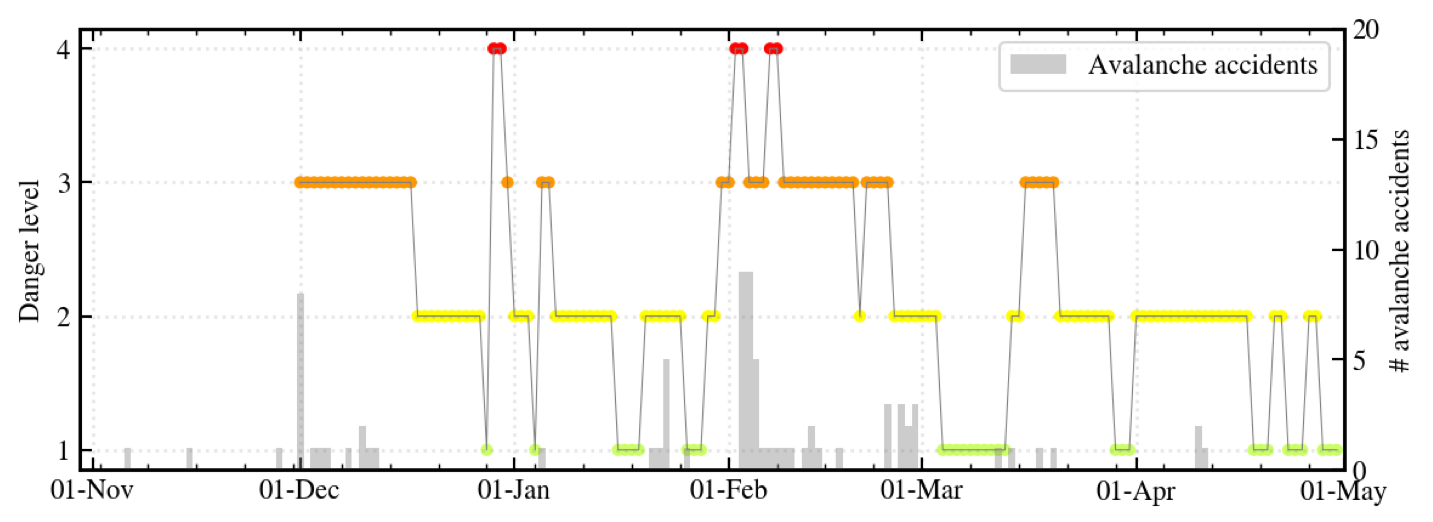
\includegraphics[width=0.8\textwidth]{Figures/figures_avapro/kalkkoegel.png}
%     \caption{Evolution of the danger level of the Micro region Kalkkoegl in the winter season 2021/22 and reporded avalanche accidents with people involvment in the grey bars }
%     \label{fig:AXLIZ_dangerlevel_evolution}
% \end{figure*}

\begin{figure*}[h]
    \centering
    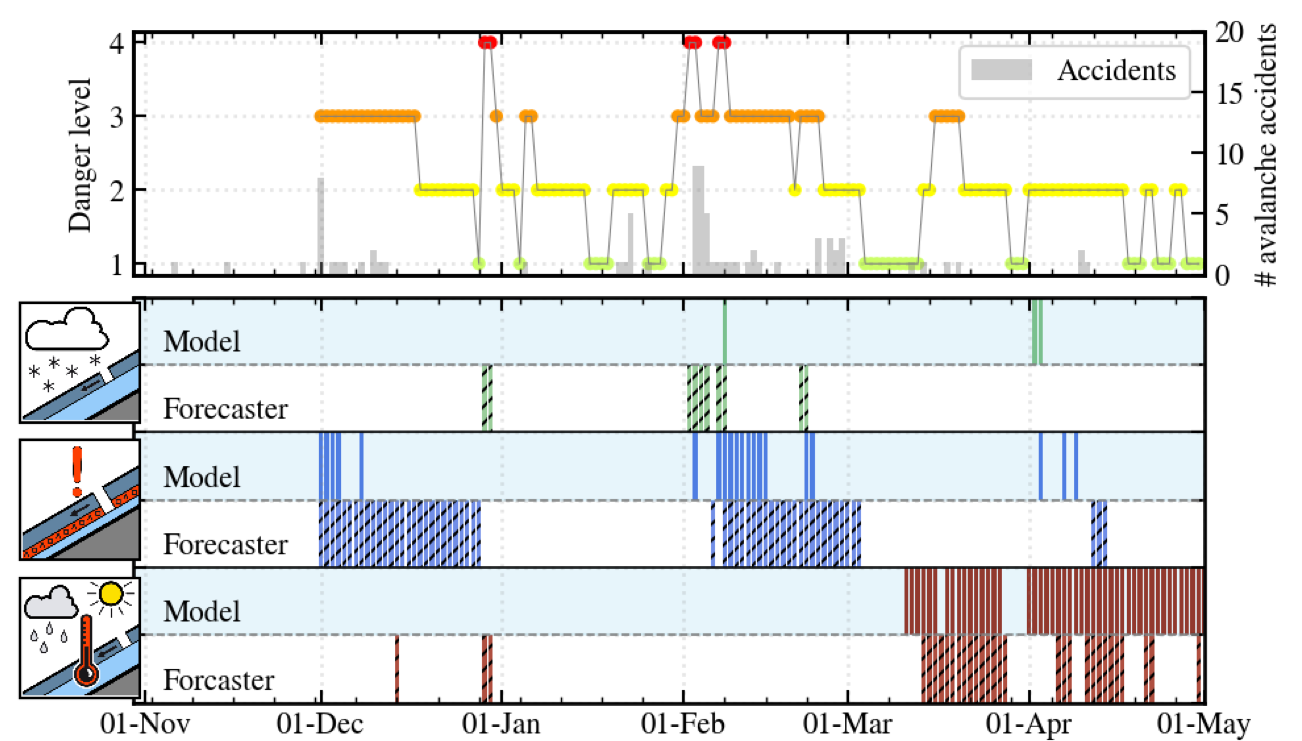
\includegraphics[width=\textwidth]{Figures/figures_avapro/AXLIZ_all.png}
    \caption{(a) Evolution of the danger level of the Micro region Kalkkoegl in the winter season 2021/22 and 
    reporded avalanche accidents with people involvment in the grey bars. (b) New Snow, Persitent Weak layer, Wet Snow Problem 
    -assigned by the algorithm for the AWS in the Axmaer Lizum in shaded area and issued problems by the LWD-Tyrol
    for the affiliated micro region Kalkkoegel}
    \label{fig:AXLIZ_dl_avaprobs}
\end{figure*}


\noindent Figure \ref{fig:AXLIZ_dl_avaprobs} (a) shows the evolution of the avalanche danger level
of the micro region \textit{Kalkkoegl} of the winterseason 2021/22 in the colored dots issued by 
the tyrolian avalanche warning service (LWD Tirol). The grey shaded bars mark the reported avalanche 
accidents. Overall it was an average winterseason with low (1) to high (4) avalanche danger level. 
There where two critical situations reaching high avalanche danger level, one at the end of december 
and one in the beginning of feburary. Especially the period in feburary was in line
with a high number of avalanche accident with wintersport recrationist envolvement. 

\noindent The assigned avalanche problem (New Snow, Persistent weaklayer, Wet Snow) is indicated by bars in the 
shaded area of Figure \ref{fig:AXLIZ_dl_avaprobs} (b) and the issued problem by the LWD-Tyrol in the 
respective lower area. 
\\
Alltogtogether the avalanche problem assignend based on simulations show a fairly similar
behavior than the subjective



\section{ vrgl stations nord /south hauptkamm}

- signifikanter cut nördlich südlich alpenhauptkamm\\
- LWD übersicht\\
- zeigen stationen ähnliches verhalten
% \begin{figure*}[ht]
%     \centering
%     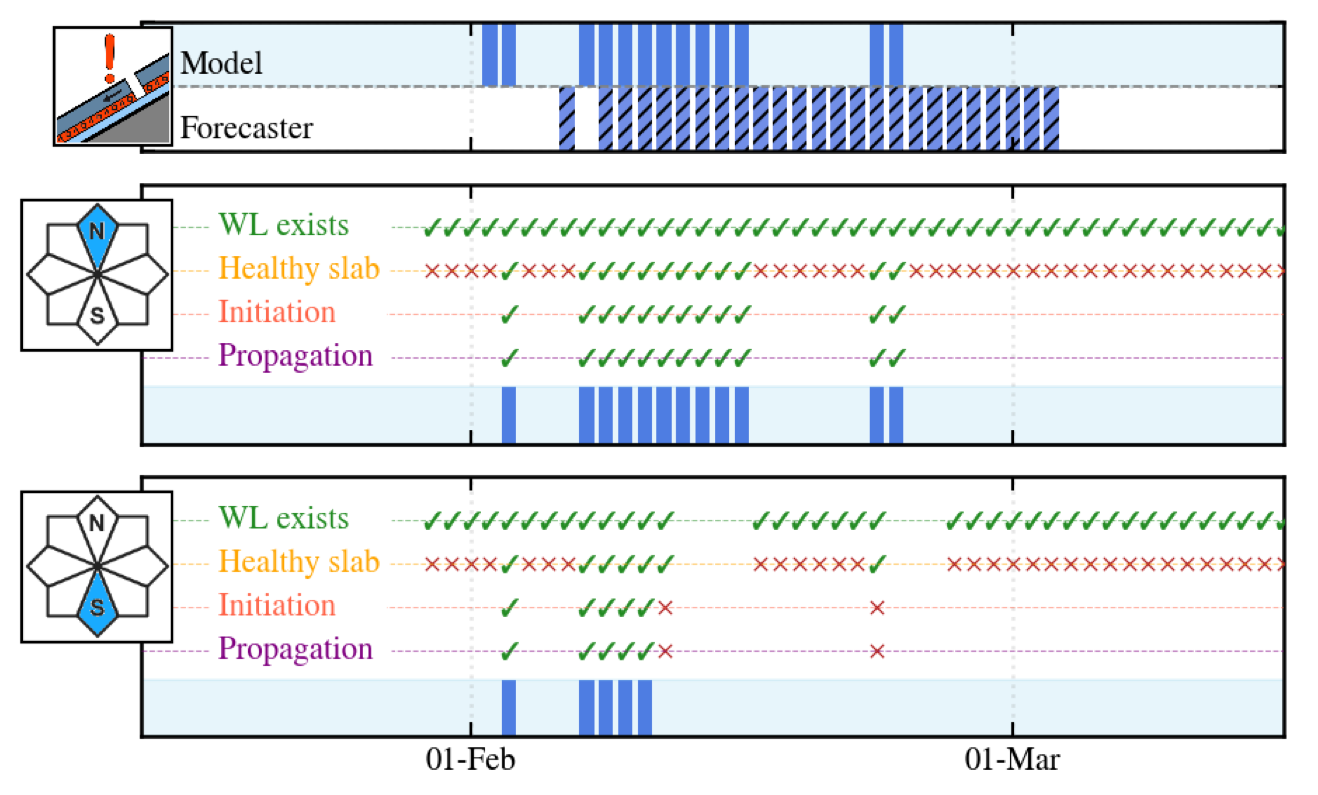
\includegraphics[width=0.8\textwidth]{Figures/figures_avapro/AXLIZ_FEB_Pers.png}
%     \caption{AXLIZ}
%     %\label{fig:}
% \end{figure*}